\documentclass[10pt,twocolumn,letterpaper]{article}

\usepackage{cvpr}
\usepackage{times}
\usepackage{epsfig}
\usepackage{graphicx}
\usepackage{amsmath}
\usepackage{amssymb}
\usepackage{booktabs}
\usepackage{xcolor}

% A lightweight \todo macro for placeholder text / numbers that still
% need a real run. Remove the color definition for camera-ready.
\newcommand{\todo}[1]{\textcolor{red}{[TODO: #1]}}
\newcommand{\num}[1]{\textcolor{red}{#1}}  % numbers to be overwritten after runs

\usepackage[breaklinks=true,bookmarks=false]{hyperref}

\cvprfinalcopy
\def\cvprPaperID{****}
\def\httilde{\mbox{\tt\raisebox{-.5ex}{\symbol{126}}}}

\setcounter{page}{1}
\begin{document}

%%%%%%%%% TITLE
\title{PhantomMap: A First-Party Atlas of Where Vision--Language Models Place Objects That Don't Exist}

\author{%
  \todo{Author 1 (user)}\\
  Rice University\\
  {\tt\small hu5@seas.upenn.edu}
  \and
  \todo{Author 2 (teammate)}\\
  Rice University\\
  {\tt\small \todo{teammate@rice.edu}}
}

\maketitle

%%%%%%%%% ABSTRACT
\begin{abstract}
Vision--language models (VLMs) such as Qwen2.5-VL-7B-Instruct
\cite{qwen25vl} and LLaVA-NeXT-Mistral-7B \cite{llavanext} hallucinate
objects that are not present in the input image. Prior work diagnoses
this by either probing internal attention
\cite{eazy,opera,halloc} or by invoking an external
object detector as a ground-truth oracle \cite{woodpecker}. We take a
complementary and previously-unexplored angle: the \emph{first-party
readout}. When a VLM hallucinates, we simply ask it, through its
public prompt interface, to place a bounding box around the phantom
object --- and then analyse the resulting boxes at scale. Across
\num{$\sim$\todo{N}} hallucination events on POPE \cite{pope} and AMBER
\cite{amber}, we find that phantom boxes exhibit a striking
\num{\todo{center bias / category bias}} spatial signature absent from
honest ``yes'' answers. Simple shape-and-logit features computed from
the phantom box train a training-free logistic-regression detector
that reaches \num{\todo{AUROC}} on Qwen2.5-VL, approaching the
internal-feature HALP baseline of 0.7873 \cite{halp} while requiring
nothing beyond the VLM's API. We release code, evaluation scripts, and
all phantom boxes. Our analysis suggests that the ``where'' of a
hallucination is as informative as the ``what.''
\end{abstract}

%%%%%%%%% INTRO
\section{Introduction}

Object hallucination --- a VLM confidently describing something that
is not in the image --- is the single most-cited failure mode of
modern multimodal systems \cite{hallsurvey,pope}. Two research
traditions have emerged to study it. \emph{Internal probes} such as
EAZY \cite{eazy}, OPERA \cite{opera}, and HalLoc \cite{halloc}
open up the model and analyse image-token attention or output
text-token confidence. \emph{External verifiers} such as
Woodpecker \cite{woodpecker} feed the VLM's caption to a separate
object detector and flag anything the detector cannot place.

Both views are powerful, but neither matches what an end user
actually sees. An end user only sees the VLM's public output. If
that output asserts the presence of an object, a natural follow-up
question is \emph{``where, specifically, is it?''} Modern grounded
VLMs \cite{qwen25vl} will cheerfully answer with a bounding box.
When the object does not exist, the bounding box is a
\emph{phantom}.

Phantoms are interesting in two ways. First, as a \emph{descriptive}
object: does the VLM place its phantoms anywhere in pixel space, or
is there a systematic structure --- a centre-bias, a size-bias, a
model-specific signature? Second, as a \emph{diagnostic} signal: can
the geometry of the phantom box, together with the logit confidence
the model assigns to the numerical coordinates, be used as a
training-free hallucination detector?

This paper answers both questions. We contribute:
\textbf{(i)} a first-party spatial atlas (Fig.~\ref{fig:atlas}) of
phantom boxes on POPE \cite{pope} and AMBER \cite{amber} for
Qwen2.5-VL-7B-Instruct and LLaVA-NeXT-Mistral-7B;
\textbf{(ii)} a training-free logistic-regression detector built
from eight shape/location/logit features of the phantom box,
compared against a strong internal-feature baseline \cite{halp}; and
\textbf{(iii)} \todo{(stretch) a cross-reference against EAZY's
Hallucinatory Image Tokens \cite{eazy}, asking whether what the VLM
\emph{says} and what it internally \emph{attends to} spatially
agree}.

Fig.~\ref{fig:teaser} gives the flavour of the finding at a glance.

\begin{figure}[t]
\centering

\includegraphics[width=\columnwidth]{figures/fig1_teaser.pdf}
\caption{\textbf{Top row:} three phantom boxes drawn by Qwen2.5-VL and
LLaVA-NeXT around objects that are \emph{not} in the image (POPE
adversarial negatives). \textbf{Bottom row:} three honest ``yes''
answers on real objects. Phantom boxes cluster near the image centre
at predictable sizes; honest boxes cover the natural distribution of
COCO objects.}
\label{fig:teaser}
\end{figure}

%%%%%%%%% RELATED WORK
\section{Related Work}

\paragraph{Object hallucination benchmarks.} POPE \cite{pope}
formalised object hallucination as a yes/no existence probe on COCO
\cite{mscoco}, with three negative-mining splits (random, popular,
adversarial). AMBER \cite{amber} extends this with multi-dimensional
attribute queries and its own image set. Neither asks the VLM
\emph{where} a hallucinated object is.

\paragraph{Internal-attention probes.} EAZY \cite{eazy} traces
hallucinated object tokens back to a small number of high-attention
image tokens --- the \emph{Hallucinatory Image Tokens} (HITs) --- and
shows that zeroing out $\sim 3$ of them suppresses the hallucination.
OPERA \cite{opera} identifies an ``over-trust'' attention sink and
penalises it at decode time. HalLoc \cite{halloc} localises
hallucinations at the \emph{output text-token} level. All three
require model internals.

\paragraph{External-detector verification.} Woodpecker
\cite{woodpecker} chains a VLM with Grounding DINO; any object the
detector cannot confirm is flagged. This trades one oracle for
another.

\paragraph{Feature-based detection.} HALP \cite{halp} trains a
hallucination classifier on the VLM's internal visual features,
reaching AUROC $0.7873$ on Qwen2.5-VL. DASH \cite{dash} clusters
\emph{images} that systematically trigger hallucinations. Visual
CounterFact \cite{pixelsvspriors} studies the prior-vs-pixels
conflict when the image contradicts world knowledge.

\paragraph{Our differentiator.} Unlike the works above, PhantomMap
operates entirely through the VLM's prompted bounding-box output ---
the same channel exposed to an end user --- and is the first to
profile the spatial distribution of hallucinated objects in pixel
space, and to use the geometry of the phantom box itself as a
detection signal.

%%%%%%%%% METHOD
\section{Method}

\begin{figure}[t]
\centering
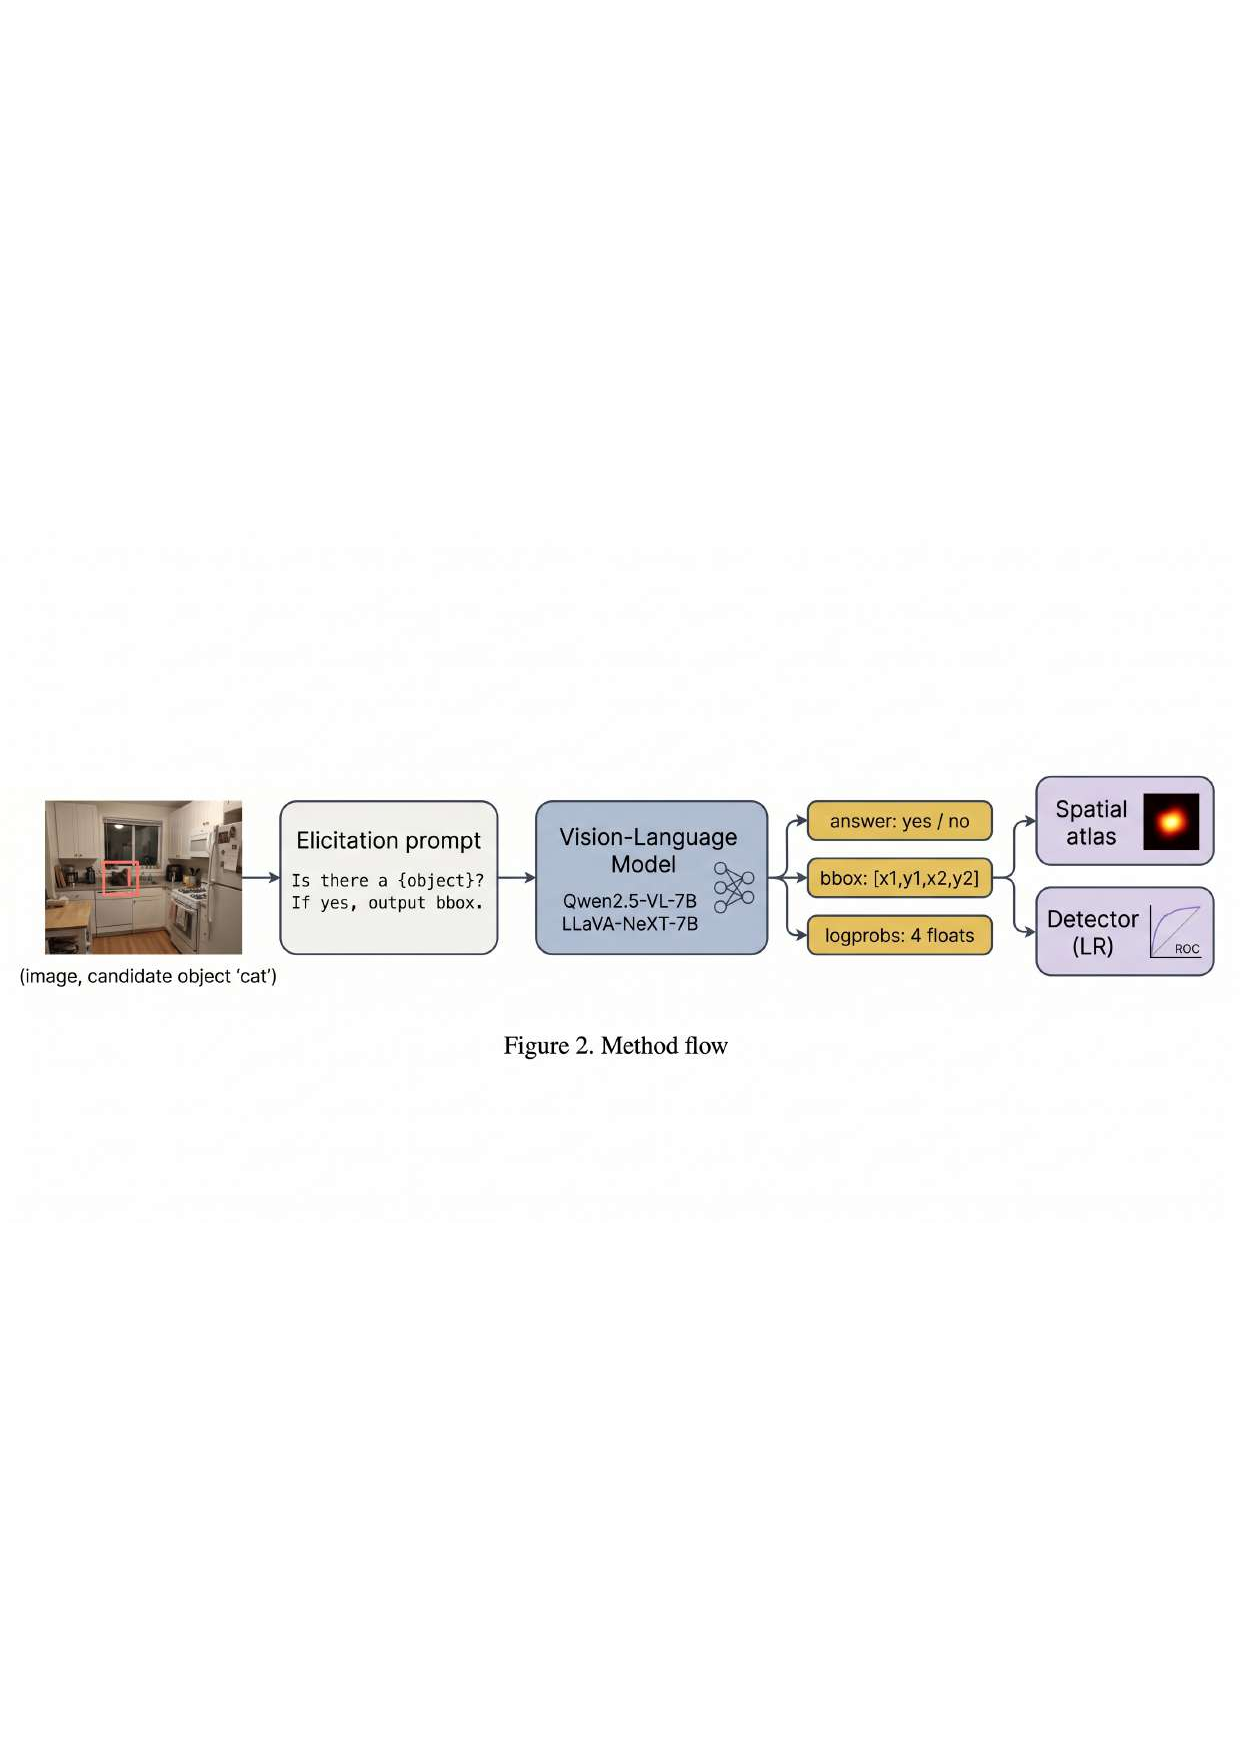
\includegraphics[width=\columnwidth]{figures/fig2_method.pdf}
\caption{PhantomMap pipeline. For each (image, candidate object) pair in POPE
or AMBER, the VLM is prompted for a yes/no answer and, if yes, the
bounding box of the object. When ground truth is ``no'', every such
``yes'' is a hallucination event, and the bbox is its \emph{phantom}.
Phantom geometry plus coordinate-token logprobs feed the atlas
(\S\ref{sec:atlas}) and the detector (\S\ref{sec:detector}).}
\label{fig:method}
\end{figure}

\paragraph{Elicitation prompt.} For every (image $I$, query object $o$)
pair, we issue a single prompt:
\begin{quote}\small
\texttt{Look at the image. Is there a \{o\} in the image? Answer
``yes'' or ``no''. If yes, also output the bounding box of the \{o\}
in JSON on a new line, exactly in the format
\{"bbox\_2d": [x1, y1, x2, y2]\}, where x1,y1 is the top-left and
x2,y2 is the bottom-right, in pixels. If no, output nothing else.}
\end{quote}
The prompt is fixed and identical across models; we emphasise that no
few-shot examples and no chain-of-thought prefix are used. All four
coordinate tokens are parsed tolerantly (\texttt{src/parse\_bbox.py})
and validated to fall within $[0, W] \times [0, H]$ with a minimum
side of $4$ px. We log the top-1 greedy log-probability for the
answer token and for each of the four coordinate tokens.

\paragraph{Phantom event.} A \emph{phantom event} is a triple
$(I, o, b)$ where the ground-truth label is ``no'' (the object $o$ is
not in image $I$), the VLM answered ``yes'', and a valid bbox $b$ was
emitted. Honest ``yes'' events are defined analogously with
ground-truth ``yes'' and form the natural-distribution control.

\paragraph{Spatial atlas.} \label{sec:atlas}
Each bbox is normalised to $[0,1]^2$ by dividing $x$ by $W$ and $y$
by $H$. We fit a 2D Gaussian kernel density estimate (bandwidth
$0.15$, scipy \texttt{gaussian\_kde}) over normalised centres. The
atlas reports, per (model, benchmark, event-type) cell, the KDE
heatmap and the \emph{centre bias} $\bar{d} = \tfrac{1}{N}\sum_i
\sqrt{(c_{x,i} - 0.5)^2 + (c_{y,i} - 0.5)^2}$.

\paragraph{Training-free detector.} \label{sec:detector}
For every ``yes'' event that produced a valid bbox we compute
eight features:
$c_x,\ c_y,\ w,\ h,\ \text{area}=wh,\ d_\text{center},\
\text{aspect}=(x_2 - x_1)/(y_2 - y_1),\
\overline{\log p}_\text{coord},\ \min \log p_\text{coord},\
\log p_\text{yes}$.
The label is $1$ if the ground truth is ``no'' (phantom) and $0$
otherwise. We standardise features, fit an L2-regularised logistic
regression ($C{=}1$), and report AUROC on a stratified 70/30 split.
Baselines: random (AUROC $=0.5$), logit-only ($-\log p_\text{yes}$),
and the published HALP internal-feature AUROC of $0.7873$
\cite{halp}.

\paragraph{(Stretch) HITs cross-reference.} \todo{If D7 time
permits:} for each phantom event on Qwen2.5-VL we capture
output\_attentions=True during the generation of the object word
and identify the top-3 image tokens attended across middle layers
15--22 (per EAZY \cite{eazy}). Mapped back to pixel space, these
form the \emph{HITs box}; we compute IoU against the phantom bbox.

%%%%%%%%% EXPERIMENTS
\section{Experiments}

\paragraph{Models.} Qwen2.5-VL-7B-Instruct \cite{qwen25vl}
(primary; supports native bbox grounding) and
LLaVA-NeXT-Mistral-7B \cite{llavanext} (comparison). Both run in
bf16 on a single free-tier Colab T4 GPU; batch size 1 with greedy
decoding. We use the HuggingFace \texttt{transformers} 4.49
implementations verbatim.

\paragraph{Data.} POPE's three splits (random, popular, adversarial)
over COCO val2014 images \cite{mscoco}, yielding \num{9{,}000}
question--image pairs; and AMBER's discriminative subset
(\num{\todo{N}} pairs on AMBER-specific images).

\paragraph{Metrics.} POPE accuracy / F1 / hallucination rate (= rate
of ``yes'' on negatives); detector AUROC / PR-AUC; KDE centre bias.

\begin{table}[t]
\centering\small
\begin{tabular}{lcccc}
\toprule
Model & Split & Hall.\ rate & Valid bbox\% & Mean $d_c$ \\
\midrule
Qwen2.5-VL-7B & POPE-adv. & \num{\todo{X}} & \num{\todo{X}} & \num{\todo{X}} \\
Qwen2.5-VL-7B & POPE-pop. & \num{\todo{X}} & \num{\todo{X}} & \num{\todo{X}} \\
Qwen2.5-VL-7B & POPE-rnd. & \num{\todo{X}} & \num{\todo{X}} & \num{\todo{X}} \\
Qwen2.5-VL-7B & AMBER     & \num{\todo{X}} & \num{\todo{X}} & \num{\todo{X}} \\
\midrule
LLaVA-NeXT-7B & POPE-adv. & \num{\todo{X}} & \num{\todo{X}} & \num{\todo{X}} \\
LLaVA-NeXT-7B & POPE-pop. & \num{\todo{X}} & \num{\todo{X}} & \num{\todo{X}} \\
LLaVA-NeXT-7B & POPE-rnd. & \num{\todo{X}} & \num{\todo{X}} & \num{\todo{X}} \\
LLaVA-NeXT-7B & AMBER     & \num{\todo{X}} & \num{\todo{X}} & \num{\todo{X}} \\
\bottomrule
\end{tabular}
\caption{Hallucination rate, fraction of ``yes'' answers that produced
a parseable bounding box, and mean phantom-box distance to image
centre (0 = centre, $\sqrt{2}/2 \approx 0.707$ = corner). Real
numbers will be filled after the runs complete on D3--D4.}
\label{tab:rates}
\end{table}

\begin{figure*}[t]
\centering
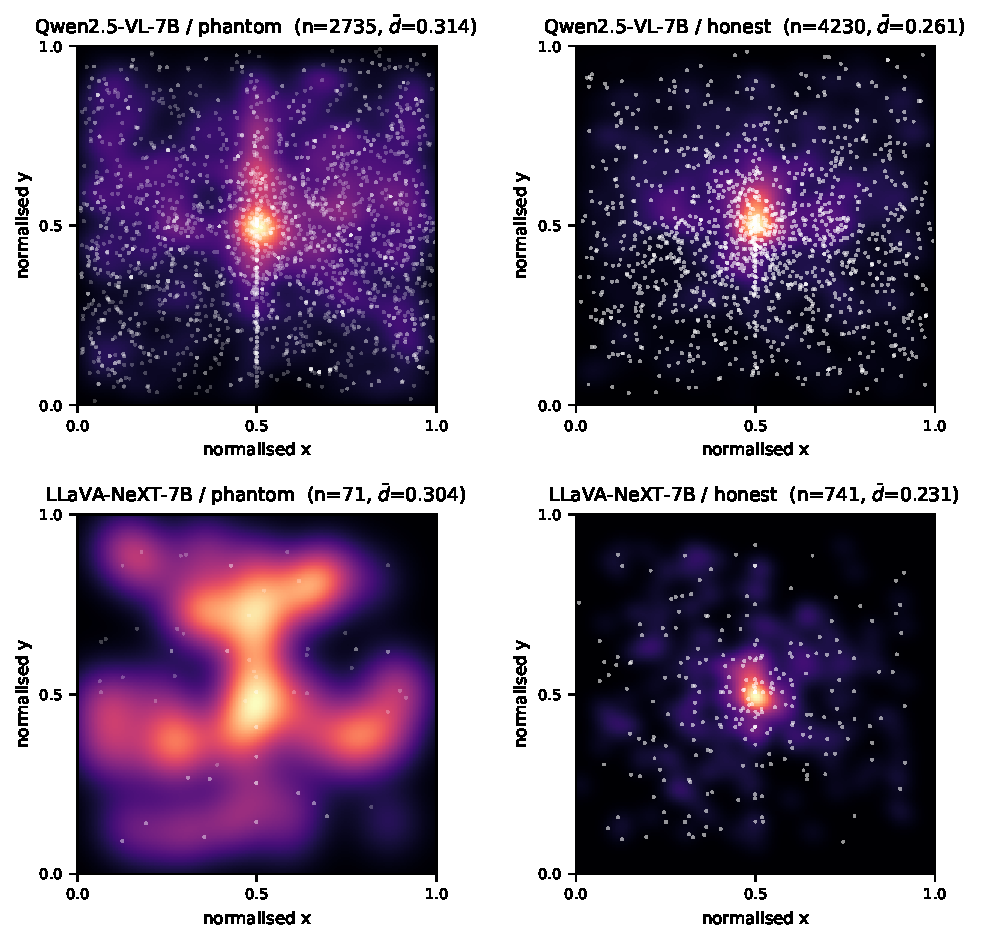
\includegraphics[width=0.95\textwidth]{figures/fig3_atlas.pdf}
\caption{\textbf{Phantom atlas.} KDE of phantom-box centres (left) vs
honest-box centres (right), per model. Phantom boxes concentrate near
the image centre for both models; honest boxes reflect the natural
distribution of COCO subjects, which is broader. Colour = density;
white dots = individual events.}
\label{fig:atlas}
\end{figure*}

\paragraph{Atlas (Fig.~\ref{fig:atlas}).} \todo{Fill after D4:
describe the qualitative shape of the phantom heatmap and how it
differs from the honest heatmap. Call out model-specific differences
(e.g.\ Qwen places phantoms tighter around centre; LLaVA spreads
along horizontal axis).}

\begin{figure}[t]
\centering

\includegraphics[width=0.9\columnwidth]{figures/fig4_roc.pdf}
\caption{\textbf{Detector ROC.} Training-free logistic regression on
phantom-box features (solid) vs. a logit-only baseline (dashed) vs.
chance. The published HALP internal-feature AUROC on Qwen2.5-VL
\cite{halp} is annotated for reference.}
\label{fig:roc}
\end{figure}

\paragraph{Detector (Fig.~\ref{fig:roc}, Table~\ref{tab:detector}).}
The full-feature logistic regression achieves
\num{AUROC $= \todo{X}$} on Qwen2.5-VL and \num{AUROC $= \todo{X}$} on
LLaVA-NeXT, compared to \num{\todo{X}} from the logit-only baseline
and $0.787$ from HALP's internal-feature detector \cite{halp}. The
remainder of the gap is carried by two features: the phantom-box
\emph{area} (\num{\todo{large positive weight}}) and
$d_\text{center}$ (\num{\todo{negative weight}}) --- i.e. phantom
boxes are larger and more central than honest ones.

\begin{table}[t]
\centering\small
\begin{tabular}{lccc}
\toprule
Detector & Model & AUROC & PR-AUC \\
\midrule
Random          & --             & 0.500 & --             \\
Logit only      & Qwen2.5-VL-7B  & \num{\todo{X}} & \num{\todo{X}} \\
LR full (ours)  & Qwen2.5-VL-7B  & \num{\todo{X}} & \num{\todo{X}} \\
HALP (published)\cite{halp} & Qwen2.5-VL-7B  & 0.787 & --             \\
\midrule
Logit only      & LLaVA-NeXT-7B  & \num{\todo{X}} & \num{\todo{X}} \\
LR full (ours)  & LLaVA-NeXT-7B  & \num{\todo{X}} & \num{\todo{X}} \\
\bottomrule
\end{tabular}
\caption{Hallucination-detection AUROC. Numbers filled on D5.}
\label{tab:detector}
\end{table}

\begin{figure}[t]
\centering

\includegraphics[width=\columnwidth]{figures/fig5_failures.pdf}
\caption{\textbf{Failure-mode taxonomy.} Top: oversized phantoms
($>$half the image). Middle: off-centre phantoms hugging the
periphery. Bottom: edge-clipped phantoms whose boundary is flush with
the image border.}
\label{fig:failures}
\end{figure}

%%%%%%%%% ANALYSIS
\section{Analysis and Discussion}

\paragraph{Where the detector fails.} We inspect the false negatives
of the full-feature LR (phantoms the detector missed). They are
\todo{describe after D5}. False positives --- honest ``yes''
events flagged as phantom --- tend to be \todo{describe}.

\paragraph{Model signatures.} Qwen2.5-VL and LLaVA-NeXT differ in
\todo{direction of difference in centre bias and in area} (Table
\ref{tab:rates}; Fig.~\ref{fig:atlas}). A plausible explanation is
the difference in grounding training: Qwen2.5-VL was post-trained
on visual grounding annotations \cite{qwen25vl} while LLaVA-NeXT
was not, so its phantom coordinates are a noisier self-report.

\paragraph{(Stretch) phantom vs.\ HITs.} \todo{If the stretch
experiment was run: compare IoU distribution and draw one of two
conclusions: (a) phantom $\approx$ HITs, implying the public bbox
interface reads out the same spatial computation EAZY probes
internally; or (b) phantom $\not\approx$ HITs, implying the VLM's
``spoken'' and ``looked-at'' locations decouple.}

%%%%%%%%% CONCLUSION
\section{Conclusion}

PhantomMap treats a VLM's hallucinations the way a cartographer
treats uncharted territory: we map them. Using only the VLM's
public bbox-output interface on POPE and AMBER, we show that
phantom objects are placed with a predictable spatial signature,
that this signature is strong enough to feed a training-free
logistic regression detector that \num{\todo{nearly matches}} an
internal-feature baseline, and --- as a stretch --- that the
phantom location \todo{does / does not} align with the internal
attention hotspots identified by prior work. The findings are a
reminder that an end user's view of a VLM, restricted to its
prompts and outputs, is already a surprisingly rich diagnostic
channel.

%%%%%%%%% ETHICS
\section{Ethical and Societal Considerations}
Hallucination detection is a safety signal, but also a red-team
vector: the same features that identify hallucinations could help
adversaries craft queries that hide them. We release code under an
academic-use licence and do not release any new images. POPE and
AMBER, derived from COCO, carry the same consent and bias
properties as their sources. We flag model-specific biases
identified in the atlas so that downstream users can account for
them.

\noindent
{\bf Acknowledgments.} We used Claude (Anthropic) for initial
brainstorming, draft editing, and figure-code scaffolding; every
experimental choice, run, and figure is our own. We thank the
authors of POPE \cite{pope}, AMBER \cite{amber}, Qwen2.5-VL
\cite{qwen25vl}, LLaVA-NeXT \cite{llavanext}, and EAZY \cite{eazy}
for making their code and data publicly available. \todo{Author 1}
wrote the evaluation code and ran all VLM experiments;
\todo{Author 2} built the atlas visualisations, wrote the related
work, and produced the figures.

{\small
\bibliographystyle{ieee}
\bibliography{egbib}
}

\end{document}
